\chapter{连通性}


\vspace{-1 em}
\section{连通空间}

\vspace{-1 em}
\begin{definition}[连通空间]
    设$X$是一个拓扑空间.如果存在非空、不相交的开集 $U$ 和 $V$，使得 $U \cup V = X$，则称$X$是\textbf{不连通的}，$\{U, V\}$ 是$X$的一个\textbf{分割}.否则，称$X$是\textbf{连通的}.
\end{definition}

\begin{instance}
    $\mathbb{R}_{fc}$ 是连通的.
    \begin{proof}
        假设$\{U,V\}$是$\mb{R}_{fc}$的一个分割，则$U\cap V=\varnothing,U\cup V=\mb{R}_{fc},U,V$均为开集.\par
        取$U=\mb{R}-\{a_1,a_2,\cdots,a_n\},V=\mb{R}-\{b_1,b_2,\cdots,b_m\}$，因此$U\cap V=\mb{R}-\{a_1,\cdots,a_n,b_1,\cdots,b_m\}$矛盾，因此$\mb{R}_{fc}$没有分割，因而连通.
    \end{proof}
\end{instance}

\begin{instance}
    $\mathbb{R}_l$ $\left(\text{基为} \left\{[a,b) \mid a<b\right\}\right)$ 是不连通的. \par
    取开集$U=(-\infty,0)=\bigcup_{n\in\mb{Z_+}}[-n,0)$和开集$V=[0,+\infty)=\bigcup_{n\in\mb{Z}_+}[0,n)$即可.
\end{instance}

\begin{proposition}
    $X$是不连通的 $\iff$ 存在$X$的一个非空、既开又闭的真子集.
\end{proposition}

\begin{instance}
    $\mathbb{E}^1$ 是连通的.
    \begin{proof}
        假设不然，则存在 $\mathbb{E}^1$ 的一个非空、既开又闭的真子集 $A$.\par
        假设 $b \notin A$ 且 $(b, +\infty) \cap A \neq \varnothing$.\par
        令 $d = \inf\{a \in A \mid a > b\}$.因为 $A$ 在 $\mathbb{E}^1$ 中是闭的，所以 $d \in A$.
        因此 $d > b$，且 $[b, d) \cap A = \varnothing$.\par
        这意味着 $d$ 不在 $A$ 的内部，所以 $A$ 不是开集.矛盾！
    \end{proof}
\end{instance}

\begin{definition}[连通子集]
    设$X$是拓扑空间，$A \subset X$.如果$A$在子空间拓扑中是连通的，则称$A$在$X$中是\textbf{连通的}（或$A$是$X$中的一个\textbf{连通子集}）.
\end{definition}

\begin{instance}
    $(-2, -1) \cup (1, 2) \subset \mathbb{E}^1$ 是不连通的.
\end{instance}

\begin{lemma}
    设$X$是一个拓扑空间，$A \subset X$.则$A$在$X$中是不连通的 $\iff$ 存在$X$中的开集 $U$ 和 $V$，使得 $U \cap A \neq \varnothing$, $V \cap A \neq \varnothing$, $U \cup V \supset A$，且 $(U \cap A) \cap (V \cap A) = \varnothing$.
    这样的 $\{U, V\}$ 称为$A$在$X$中的一个\textbf{分割}.
\end{lemma}
\begin{figure}[h]
    \centering
    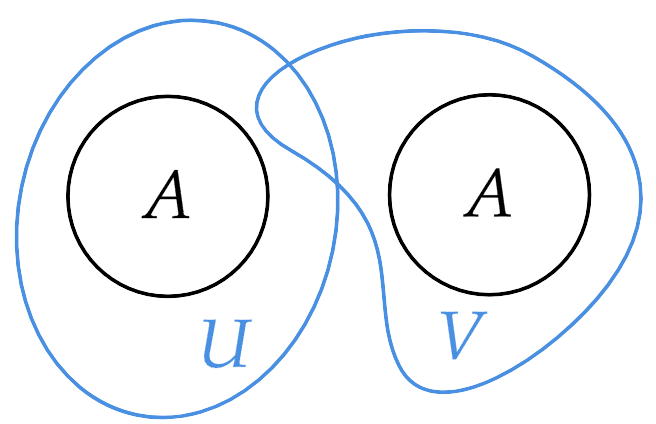
\includegraphics[width=0.3\textwidth]{fig/7.1.png}
    \captionof{figure}{}
\end{figure}


\begin{proposition}
    连通空间的连续像是连通的.即若 $f: X \to Y$ 是连续函数且 $X$ 是连通空间，则 $f(X)$ 在 $Y$ 中是连通的.
\end{proposition}
\begin{proof}
    假设不然，则存在 $f(X)$ 在 $Y$ 中的一个分割 $\{U, V\}$，即 $U$ 和 $V$ 都是开集，$U \cap f(X) \neq \varnothing$, $V \cap f(X) \neq \varnothing$, $U \cup V \supset f(X)$，且 $U \cap V \cap f(X) = \varnothing$.\par
    因为 $U \cap f(X) \neq \varnothing$ 且 $V \cap f(X) \neq \varnothing$，所以 $f^{-1}(U)$ 和 $f^{-1}(V)$ 在 $X$ 中都是非空开集.\par
    因为 $U \cap V \cap f(X) = \varnothing$，所以 $f^{-1}(U) \cap f^{-1}(V) = f^{-1}(U \cap V) = \varnothing$.\par
    因为 $f(X) \subset U \cup V$，所以 $f^{-1}(U) \cup f^{-1}(V) = X$.\par
    因此$\{f^{-1}(U),f^{-1}(V)\}$是$X$的一个分割，所以 $X$ 是不连通的，矛盾！
\end{proof}

\begin{theorem}
    设 $X_1 \cong X_2$.$X_1$ 是连通的 $\iff X_2$ 是连通的.
\end{theorem}
这个定理表示连通性是拓扑性质，因此可以考查两个拓扑的连通性来判定它们是否是同胚的.如果两个拓扑空间一个连通一个不连通，则它们一定不是同胚的.

\begin{instance}
    $\mathbb{E}^1 \not\cong \mathbb{R}_l$.
\end{instance}

\begin{instance}
    $A \subset \mathbb{E}^1$，$A$ 是连通的 $\iff A$ 是一个区间.
\end{instance}
\begin{proof}
    “$\Rightarrow$” 如果 $A$ 不是一个区间，那么存在 $x$，使得 $x \notin A$，$A \cap (-\infty, x) \neq \varnothing$，$A \cap (x, +\infty) \neq \varnothing$.\par
    因此 $\{(-\infty, x), (x, +\infty)\}$ 是 $A$ 在 $\mathbb{E}^1$ 中的一个分割.矛盾！ \par
    “$\Leftarrow$” $(a, b), (a, +\infty), (-\infty, b)$ 都与 $\mathbb{E}^1$ 同胚，因此都是连通的.\par
    $[a, b]$ 是连通的，考虑函数 $f: \mathbb{E}^1 \to \mathbb{E}^1$，$x \mapsto \begin{cases} a, & x<a \\ x, & a \leq x \leq b \\ b, & x>b \end{cases}$.它是连续的，因此其像 $[a,b]$是连通的.\par
    $[a,+\infty)$是连通的，考虑函数 $f: \mathbb{E}^1 \to \mathbb{E}^1$，$x \mapsto \begin{cases}
        x , x\geq a\\
        2a-x,x\leq a
    \end{cases}$.它是连续的，因此其像 $[a,+\infty)$ 是连通的.\par
    因为$[a,b) \cong (a,b] \cong (-\infty,b] \cong [a, +\infty) $，$[a,b),(a,b],(-\infty,b]$是连通的
\end{proof}

\begin{theorem}[介值定理]
    设$X$是一个连通拓扑空间，$f: X \to \mathbb{E}^1$ 是连续的，$x_0, x_1 \in X$ 且 $f(x_0) < f(x_1)$.那么对于任意 $y \in \left[f(x_0), f(x_1)\right]$，都存在 $x \in X$，使得 $f(x) = y$.
\end{theorem}
上述定理和极值定理一样，实则是拓宽了在数学分析中学习的连续函数在有界闭区间上取值的性质.其原因在于欧式空间下有界闭区间是连通的紧集.



\begin{lemma}
    设$X$是一个拓扑空间，$A\subset X$，$\{U,V\}$是$X$的一个分割，则要么$A\subset U$，要么$A\subset V$.
\end{lemma}
\begin{proof}
    如若不然，则$A\cap U \neq \varnothing,A\cap V \neq \varnothing$，因此$\{U,V\}$是$A$在$X$中的一个分割，所以$A$是不连通的.矛盾！
\end{proof}


\begin{lemma}[引理7.2的一般形式]{7.3}
    设 $X$ 是拓扑空间，$A\subset B\subset X$，$\{U,V\}$ 是 $B$ 在 $X$ 中的一个分割.若 $A$ 在 $X$ 中是连通的，则要么 $A\subset U$，要么 $A\subset V$.
\end{lemma}
\begin{proof}
    使用反证法，假设$A\cap U\neq\varnothing$ 且 $A\cap V\neq\varnothing$.\par
    \begin{wrapfigure}{r}{0.25\textwidth}
        \vspace{-3 em}
        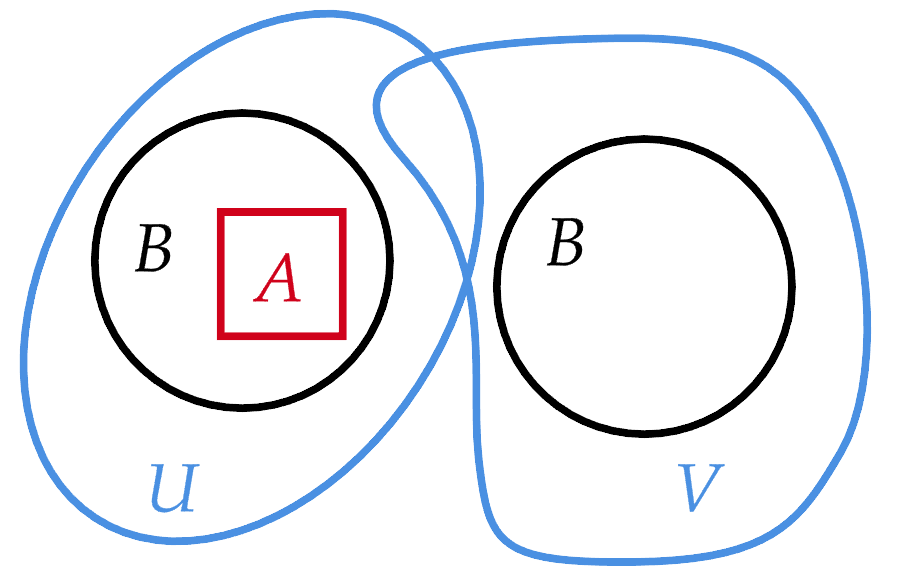
\includegraphics[width=0.25\textwidth]{fig/7.2.png}
        \captionof{figure}{}
        \vspace{-1 em}
    \end{wrapfigure}
    于是 $\{U,V\}$ 给出了 $A$ 在 $X$ 中的一个分割，说明 $A$ 不连通，矛盾.\par
    因此必有 $A\cap U=\varnothing$ 或 $A\cap V=\varnothing$.\par
    这两个条件就等价于要么$A\subset U$，要么$A\subset V$.
\end{proof}
\vspace{1 em}

\begin{proposition}[连通子集的闭包连通]
    设 $X$ 是一个拓扑空间，$A$ 是 $X$ 中的一个连通子集，$B\subset X$且$A\subset B\subset \overline{A}$.则 $B$ 是连通的.特别地 $\overline{A}$ 是连通的.
\end{proposition}
\begin{proof}
    反证法，如若不然，则存在 $B$ 在 $X$ 中的一个分割 $\{U,V\}$.\par
    由引理\ref{lem:7.3}知 $A\subset U$ 或 $A\subset V$.不失一般性，不妨设 $A\subset V$，则 $A\cap U=\varnothing$.\par
    取任意$x\in U\cap B$，则 $x\in B\subset \overline{A}\Rightarrow x\in\overline{A}$.\par
    $x\in U,A\cap U=\varnothing\Rightarrow x\notin \overline{A}$，矛盾!
\end{proof}

\begin{remark}
    由 $\overline{A}=A\cup A'$可见，若向 $A$ 添入它的极限点，不会破坏连通性.
\end{remark}
\begin{instance}
    圆周$S^1=\mb{E}^1\cup\{\infty\}=\overline{\mb{E}^1}$同胚于一维欧式空间的单点紧化.由$\mb{E}^1$连通可得$S^1$连通.
\end{instance}

\begin{lemma}[交集非空的连通族的并连通]{7.4}
    设 $X$ 是拓扑空间，$\{C_\lambda\}_{\lambda\in\Lambda}$ 是一族在 $X$ 中连通的子集，且 $\bigcap_{\lambda\in\Lambda} C_\lambda \neq \varnothing$.则$\bigcup_{\lambda\in\Lambda} C_\lambda$ 是连通的.
\end{lemma}
\begin{proof}
    反证法，如若不然，则在$X$中有$\bigcup_{\lambda\in\Lambda}{C_\lambda}$分割 $\{U,V\}$.\par
    任取$\lambda$，由于 $C_\lambda$ 连通，要么$C_\lambda\subset U$，要么$C_\lambda\subset V$.\par
    由于$\bigcap_{\lambda\in\Lambda}{C_\lambda}\neq\varnothing$，取$x\in \bigcap_{\lambda}C_\lambda$，则要么$x\subset U$，要么$x\subset V$.\par
    不妨设 $x\in U$，则$\forall\, \lambda$，$C_\lambda\subset U$，则$\bigcup_{\lambda}C_\lambda\subset U$ 且 $\left(\bigcup_{\lambda}C_\lambda\right)\cap V=\varnothing$，与$\{U,V\}$是分割矛盾.
\end{proof}
该引理的想法是，如果每个子集都连通，且相互“连接”在一起(即交集非空)，则并集也连通.

\begin{theorem}[乘积空间的连通性]
    设 $X,Y$ 为拓扑空间，则 $X\times Y$ 连通当且仅当 $X$ 与 $Y$ 都连通.
\end{theorem}
\begin{proof}
    “$\Rightarrow$”投影 $\pi_X: X\times Y\to X$ 与 $\pi_Y: X\times Y\to Y$ 连续满射，连续像连通，故 $X,Y$ 连通.\par
    “$\Leftarrow$” 取任意固定点 $x_0\in X$，$\{x_0\}\times Y\cong{Y}$连通.\par
    \begin{wrapfigure}{r}{0.27\textwidth}
        \vspace{-3 em}
        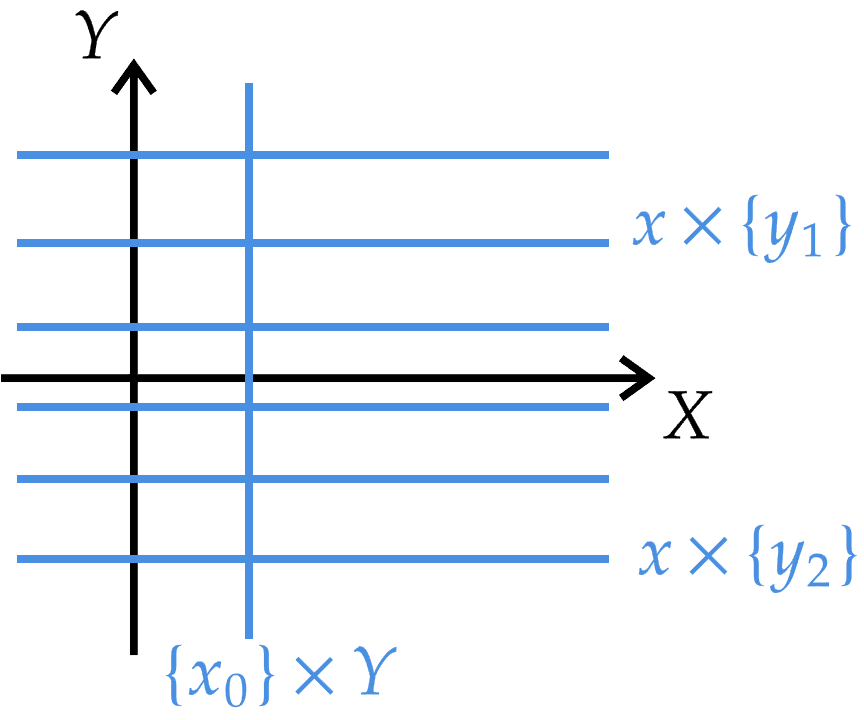
\includegraphics[width=0.27\textwidth]{fig/7.3.png}
        \captionof{figure}{}
        \vspace{-1 em}
    \end{wrapfigure}
    $\forall\,y\in Y$，$X\times\{y\}\cong X$，故连通.\par
    记$C_y:= (X\times\{y\})\cup(\{x_0\}\times Y)$ 连通，由引理\ref{lem:7.4}，$C_y$连通.\par
    $X\times Y=\bigcup_{y\in Y} C_y$，且 $\bigcap_{y\in Y} C_y=\{x_0\}\times Y\neq\varnothing$.由引理\ref{lem:7.4}，$X\times Y$ 连通.
\end{proof}
\vspace{2 em}

这个定理的结论是自然的，并且应用数学归纳法可以将其推广到有限乘积拓扑空间的情形.

\begin{corollary}[有限乘积空间的连通性]
    若 $X_1,\dots,X_n$ 为拓扑空间，则 $X_1\times\cdots\times X_n$ 连通 $\iff$ 每个 $X_i$ 连通.
\end{corollary}
\begin{instance}
    $\mathbb{E}^n=\mathbb{E}^1\times\cdots\times\mathbb{E}^1$ 连通.
\end{instance}
\begin{instance}
    $S^n=\mathbb{E}^n\cup\{\infty\}=\overline{\mathbb{E}^n}$ 连通.
\end{instance}
\section{连通分支}

\begin{definition}[连通分支]
    设$X$是一个拓扑空间，$x,y\in X$，若存在一个连通子集 $C_{x,y}\subset X,\st x,y\in C$，则定义$x\sim_c y$，那么$\sim_c$是 $X$ 上的一个等价关系，即
    \begin{enumerate}[(i)]
        \item $x\sim_c x$
        \item $x\sim_c y\Rightarrow y\sim_c x$
        \item $x\sim_c y,y\sim_c z\Rightarrow x\sim_c z$
    \end{enumerate}
    “$\sim_c$”的每一个等价类称为 $X$ 的一个\textbf{连通分支}.
\end{definition}
\begin{proof}
    下面证明$\sim_c$是一个等价关系.(i)(ii)显然成立.\par
    现证明(iii).\par
    设 $x\sim_c y,y\sim_c z$，则存在连通子集 $C_{x,y},C_{y,z}\subset X$，使得 $x,y\in C_{x,y}$，$y,z\in C_{y,z}$.\par
    因为$C_{x,y}\cap C_{y,z}\neq\varnothing$，因此$C_{x,y}\cup C_{y,z}$ 连通，故 $x\sim_c z$.
\end{proof}

    


\begin{remark}
    每个连通子集都包含于某个连通分支.
\end{remark}

一个连通分支有以下几个重要性质，即连通分支是连通的、极大的、闭的.\par

\begin{lemma}[连通分支是连通的]
    设 $C$ 是 $X$ 的一个连通分支，则 $C$ 是连通的.
\end{lemma}
\begin{proof}
    取 $x_0\in C$.$\forall\,p\in C$，存在一个连通子集$C_p\subset X$，使得 $x_0,p\in C_p$.\par
    由定义可知$C_p\subset C$，因此$C=\bigcup_{p\in C}{C_p}$.\par    
    因为$\bigcap_{p\in C} C_p\supset\{x_0\}\neq\varnothing$，由引理\ref{lem:7.4}，$C=\bigcup_{p\in C} C_p$ 连通.
\end{proof}

\begin{lemma}[连通分支的极大性]
    设 $C$ 是 $X$ 的一个连通分支，$A\subset X$ 是连通子集且 $C\subset A$，则 $A=C$.
\end{lemma}
\begin{proof}
    只需证明$A\subset C$.取$x_0\in C\subset A$.由$A$是连通子集，故$\forall\, a\in A,a\sim_c x_0$，因此$a\in C$，则$A\subset C$.
\end{proof}

\begin{lemma}[连通分支是闭集]
    若 $C$ 是 $X$ 的一个连通分支，则 $C$ 在 $X$ 中闭.
\end{lemma}
\begin{proof}
   由于$C$是连通分支，$C$连通，因此$\overline{C}$ 连通.\par
   又$C\subset \overline{C}$.由连通分支的极大性得到 $C=\overline{C}$，故 $C$ 闭.
\end{proof}

\begin{instance}
    在 $\mathbb{R}_l$（基为 $\{[a,b)\mid a<b\}$）中，任一单点集是一个连通分支.\par
    事实上，若 $x<y$，且假设$x\sim_c y$，则在连通子集 $A\subset \mathbb{R}_l$ 使得 $x,y\in A$.\par
    任取$z\in(x,y)$，则 $\{(-\infty,z),[z,+\infty)\}$ 给出 $A$ 在 $\mathbb{R}_l$ 中的一个分割，矛盾.
\end{instance}

\begin{instance}
    在 $\mathbb{Q}\subset \mathbb{E}^1$ 中，任一单点集是一个连通分支.因为我们可以在任意两个有理数中找到一个无理数将其分开.\par
    一般地，若 $X$ 的每个单点集都是一个连通分支，则称 $X$ \textbf{完全不连通(totally disconnected)}.
\end{instance}



\section{道路连通}

\begin{definition}[道路]
    在拓扑空间 $X$ 中，称从 $x$ 到 $y$ 的一条\textbf{道路}为一个连续映射 $a:[0,1]\to X$，满足 $a(0)=x$，$a(1)=y$.
\end{definition}
\begin{figure}[h]
    \centering
    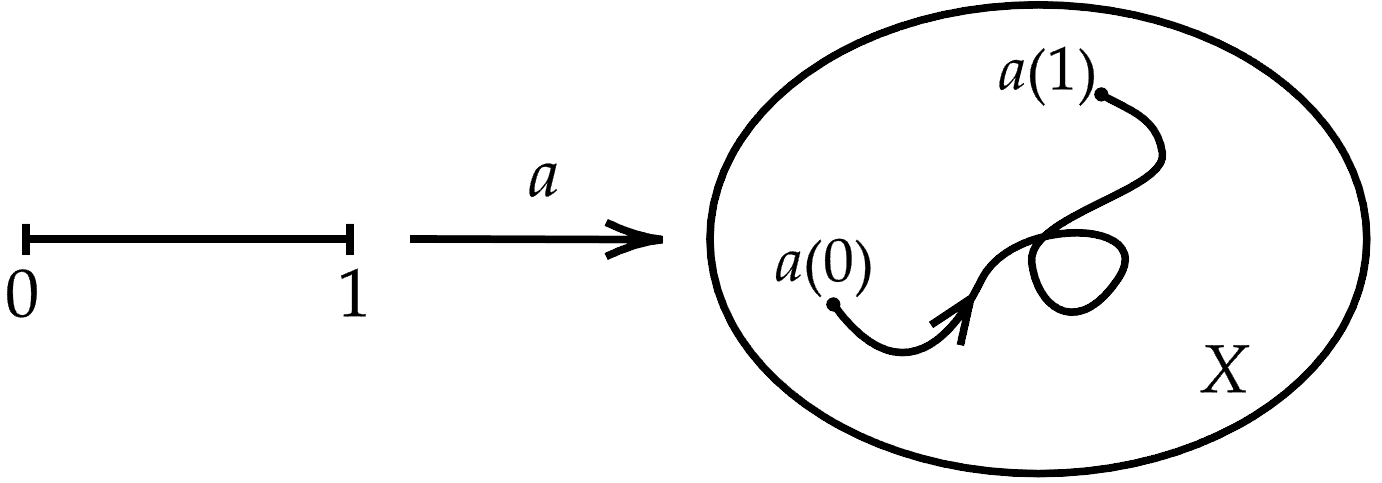
\includegraphics[width=0.6\textwidth]{fig/7.4.png}
    \captionof{figure}{道路}
\end{figure}
\begin{remark}
    一条道路不仅仅是它的像，还包含参数化信息.
\end{remark}

\begin{definition}[道路连通]
    在拓扑空间$X$中，若对任意 $x,y\in X$，都存在从 $x$ 到 $y$ 的道路，则称 $X$ 是\textbf{道路连通}的.\par
    若 $A\subset X$ 在子空间拓扑中是道路连通的，则称 $A$ 是 $X$ 的一个\textbf{道路连通子集}.
\end{definition}
需要注意，道路连通子集不能使用大空间中的道路来连接其内的两点，而必须使用子空间拓扑下的道路，因此没有类似于紧致子集和连通子集的使用大空间中集合的性质来证明其紧致性和连通性的结论.

\begin{instance}
    $\mathbb{E}^n$ 是道路连通的.给定 $x,y\in\mathbb{E}^n$，取 $a(t)=(1-t)x+ty$ 即得一道路.
\end{instance}

\begin{instance}
    $\mathbb{R}_{fc}$ 是道路连通的.\par
    \begin{wrapfigure}{r}{0.25\textwidth}
        \vspace{-3 em}
        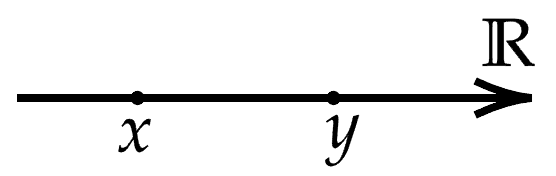
\includegraphics[width=0.25\textwidth]{fig/7.5.png}
        \captionof{figure}{}
        \vspace{-1 em}
    \end{wrapfigure}
    对任意 $x,y\in\mathbb{R}$，映射 $a:[0,1]\to\mathbb{R}$，$t\mapsto (1-t)x+ty$ 是连续的，将其视作到 $\mathbb{R}_{fc}$ 的映射仍为一条从 $x$ 到 $y$ 的道路.
\end{instance}

\begin{proposition}[连续映射保持道路连通性]
    若 $X$ 道路连通且 $f:X\to Y$ 连续，则 $f(X)$ 在 $Y$ 中是道路连通的.
\end{proposition}
\begin{proof}
    任取 $y_0,y_1\in f(X)$，取 $x_0\in f^{-1}(y_0)$，$x_1\in f^{-1}(y_1)$.\par
    由 $X$ 的道路连通性，存在从 $x_0$ 到 $x_1$ 的道路 $a:[0,1]\to X$.\par
    则 $f\circ a:[0,1]\to Y$ 是从 $y_0$ 到 $y_1$ 的道路，其像包含于 $f(X)$，故 $f(X)$ 道路连通.
\end{proof}

\begin{theorem}
    若 $X_1\cong X_2$，则 $X_1$ 道路连通当且仅当 $X_2$ 道路连通.
\end{theorem}
这告诉我们道路连通性和连通性一样，也是一个拓扑性质. 

\section{道路连通分支}

\begin{definition}[道路连通分支]
    设$X$是一个拓扑空间，$x,y\in X$，若存在一条从 $x$ 到 $y$ 的道路，则定义$x\sim_p y$，那么$\sim_p$是 $X$ 上的一个等价关系，即
    \begin{enumerate}[(i)]
        \item $x\sim_p x$
        \item $x\sim_p y\Rightarrow y\sim_p x$
        \item $x\sim_p y,y\sim_p z\Rightarrow x\sim_p z$
    \end{enumerate}
    “$\sim_p$”的每一个等价类称为 $X$ 的一个\textbf{道路连通分支}.
\end{definition}
\begin{proof}
    下面证明$\sim_p$是一个等价关系.\par
    (i)\; $x\sim_p x$.\par
    定义$\setjot[-6]\begin{aligned}[t]
            a:[0,1]&\to X \\
            t&\mapsto x
        \end{aligned}$即可，它称为常值道路.\par
        \begin{wrapfigure}{r}{0.25\textwidth}
            \vspace{-2 em}
            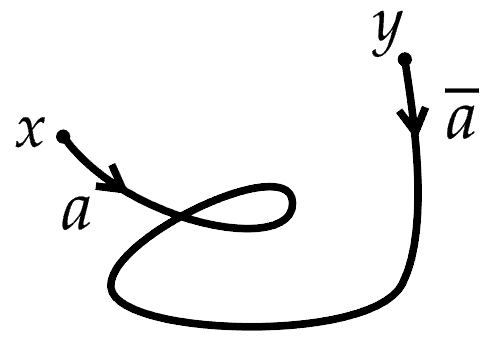
\includegraphics[width=0.25\textwidth]{fig/7.6.png}
            \captionof{figure}{逆道路}
            \vspace{-4 em}
        \end{wrapfigure}

    (ii)\;$x\sim_p y\Rightarrow y\sim_p x$.\par
    由$x\sim_p y$，可知有从$x$ 到 $y$ 的道路$a:[0,1]\to X,a(0)=x,a(1)=y$.\par
    定义$\setjot[-6]\begin{aligned}[t]
            \overline{a}:[0,1]&\to X \\
            t&\mapsto a(1-t)
        \end{aligned}$，则$\overline{a}(0)=a(1)=y,\overline{a}(1)=a(0)=x$.\par
        故$\overline{a}$是从$y$到$x$的道路，因此$y\sim_p x$.\par
    \begin{wrapfigure}{r}{0.25\textwidth}
        \vspace{-1 em}
        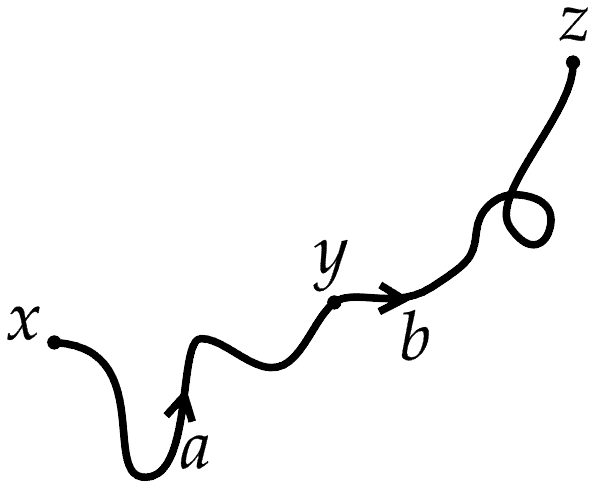
\includegraphics[width=0.25\textwidth]{fig/7.7.png}
        \captionof{figure}{乘积道路}
        \vspace{-1 em}
    \end{wrapfigure}
    (iii)\;$x\sim_p y,y\sim_p z\Rightarrow x\sim_p z$\par
    首先有$\setjot[-4]\begin{aligned}[t]
        a:[0,1] &\to X,a(0)=x,a(1)=y\\
        b:[0,1] &\to X,b(0)=y,b(1)=z
    \end{aligned}$.\par
    定义$\begin{aligned}[t]
        c:[0,1]&\to X \\
        t &\mapsto\begin{cases}
                a(2t),&0\leq t\leq\tfrac{1}{2}\\
                b(2t-1),&\tfrac{1}{2}\leq t\leq 1
            \end{cases}
    \end{aligned}$\par
    由粘贴引理知 $c$ 连续，故 $c$ 是从 $x$ 到 $z$ 的道路.
\end{proof}

\begin{lemma}[道路连通分支是道路连通的]
    $X$ 的任一道路连通分支 $P$ 都是道路连通的.
\end{lemma}
\begin{proof}
    $\forall\, x,y\in P$，由定义，存在道路$a:[0,1]\to X$ 使得 $a(0)=x$，$a(1)=y$.\par
    对任意 $t\in[0,1]$，构造$\setjot[-2]\begin{aligned}[t]
        a\circ h:[0,1] &\stackrel{h}{\to}& &[0,1]& &\stackrel{a}{\to} X \\
        s &\mapsto& &st& &\mapsto a(st)
    \end{aligned}$，它是从$a(0)$到$a(t)$的道路，因此有$a(t)\in P$，从而 $a\left([0,1]\right)\subset P$.因此 $P$ 道路连通.
\end{proof}

\begin{lemma}[道路连通分支的极大性]
    若 $P$ 是 $X$ 的一个道路连通分支，$A\subset X$ 是道路连通子集且 $P\subset A$，则 $A=P$.
\end{lemma}
\begin{proof}
    只需证明$A\subset P$.$\forall\, a\in A$，任取$x_0\in P\subset A$.由$A$道路连通性，故存在$f:[0,1]\to A\subset X,\st f(0)=a,f(1)=x_0$，即$a\sim_p x_0$.\par
    因此$a\in P$，则$A\subset P$.
\end{proof}



\section{连通与道路连通}

\begin{proposition}[道路连通必连通]
    若拓扑空间 $X$ 道路连通，则 $X$ 连通.
\end{proposition}
\begin{proof}
    反证法，假设$X$道路连通但不连通，则存在$X$的分割 $\{U,V\}$.\par
    取 $x\in U$，$y\in V$.由于 $X$ 道路连通，存在一个从$x$到$y$的道路 $a:[0,1]\to X,\st a(0)=x$，$a(1)=y$.则 $0\in a^{-1}(U)\neq\varnothing$ 与 $0\in a^{-1}(V)\neq\varnothing$.\par
    又$a^{-1}(U)\cap a^{-1}(V)=\varnothing$，$a^{-1}(U)\cup a^{-1}V=[0,1]$且$U,V$是 $[0,1]$中开集，因此$\left\{a^{-1}(U),a^{-1}(V)\right\}$是$[0,1]$ 的分割，与$[0,1]$ 连通矛盾!
\end{proof}
\begin{remark}
    上述命题的逆命题不成立，即连通空间不一定道路连通.拓扑学家正弦曲线 $X$ 即为反例.
\end{remark}

设$X=\left\{(0,y)\in\mb{E}^2|-1\leq y\leq 1\right\} \cup\left\{\, \left(x,\,\sin\frac{1}{x}\right)\in\mb{E}^1\Big| 0<x\leq 1 \,\right\}\subset \mathbb{E}^2.$\par

记 $A=\left\{(0,y)\in\mb{E}^2|-1\leq y\leq 1\right\}$，$B=\left\{\, \left(x,\,\sin\frac{1}{x}\right)\in\mb{E}^1\Big| 0<x\leq 1 \,\right\}$.
\begin{figure}[h]
    \centering
    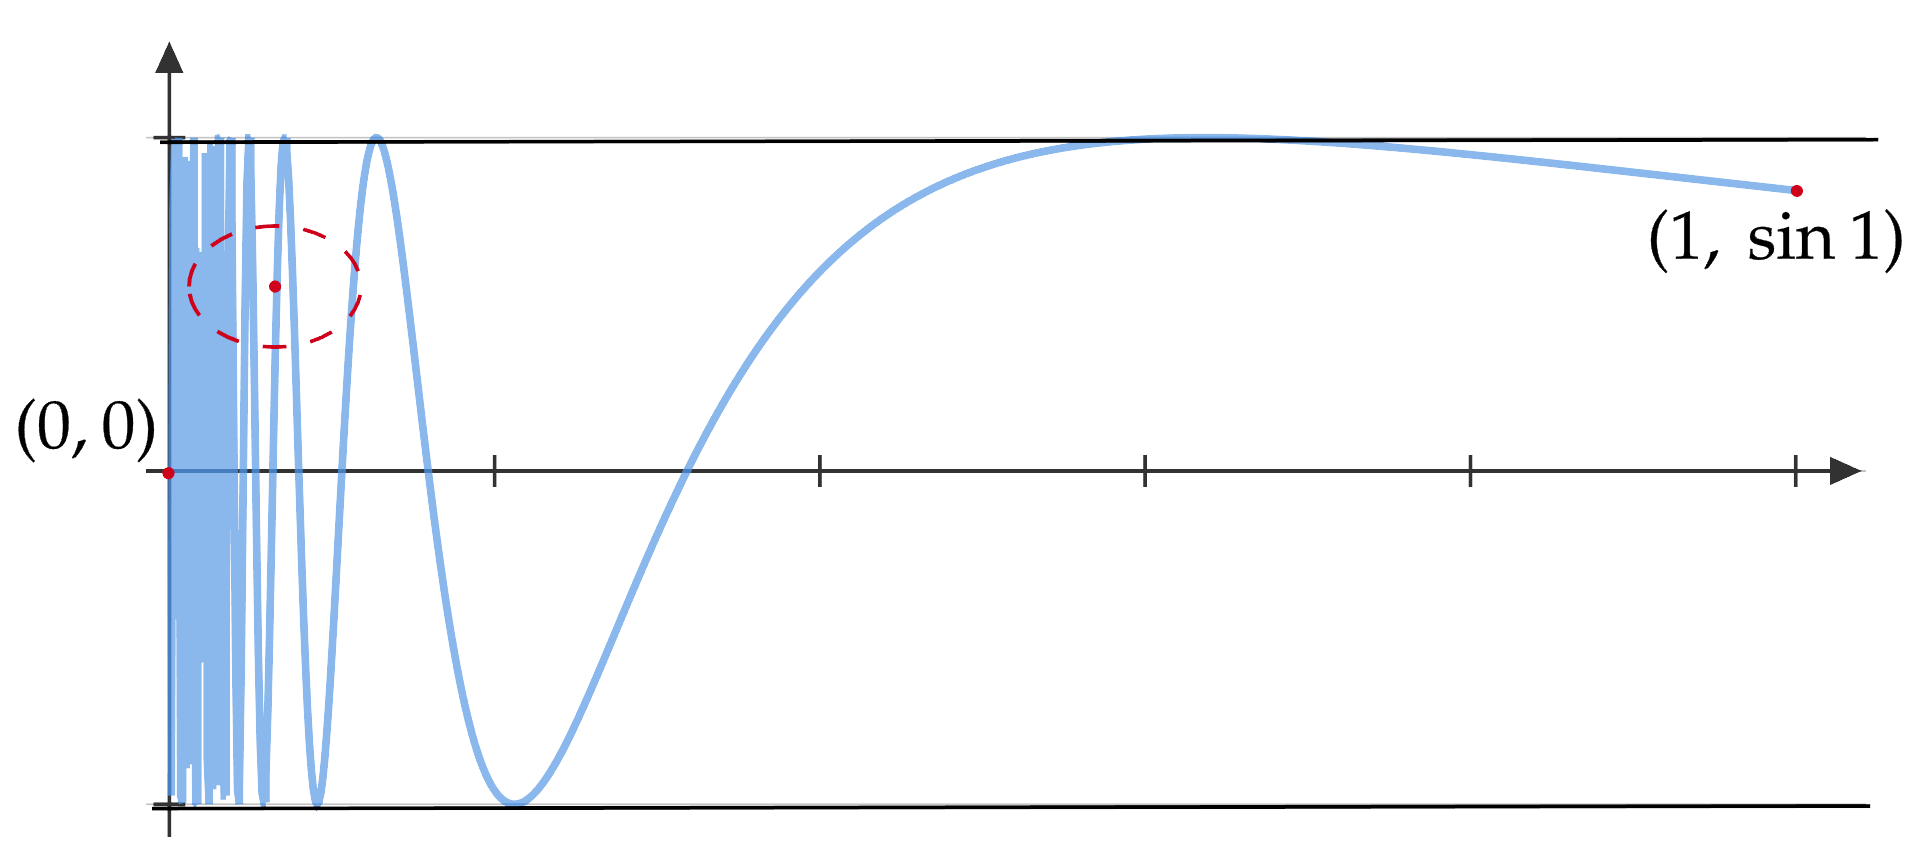
\includegraphics[width=0.7\textwidth]{fig/7.8.png}
    \captionof{figure}{拓扑学家正弦曲线}
\end{figure}\par
\begin{proof}
首先证明$X$是连通的.\par
$B$是连通的，因为$B\cong (0,1]$，那么$X=\overline{B}$也是连通的.\par
下面证明$X$不是道路连通的.\par
使用反证法，假设存在一条道路$f:[0,1]\to X,\st f(0)=(0,0)\in A$ 且 $f(1)=(1,\sin 1)\in B$.\par
注意 $A$ 在 $X$ 中是闭集，故 $f^{-1}(A)$ 为 $[0,1]$ 中闭集.令 $b=\max f^{-1}(A)$，则 $f(b)\in A$，且 $f((b,1])\subset B$.\par
令 $h=\setjot[-2]\begin{aligned}[t]
    f\circ g:[0,1] &\stackrel{g}{\to}& &[b,1]& &\stackrel{f}{\to} X \\
        t &\mapsto& &(1-t)b+t& &\mapsto \left(x(t),y(t)\right)
\end{aligned} $\par
则$h(0)=f(b)=\left(x(0),y(0)\right)=(0,y(0))\in A$，$h(t)=\left(x(t),y(t)\right)\in B$ 对 $t\in(0,1]$ 成立.
\begin{claim}{$\forall\,n\in\mathbb{Z}_{>0}$，$\exists\,t_n\in\left(0,\frac{1}{n}\right)$，使得 $h(t_n)=\big(x(t_n),\,y(t_n)\big)$ 满足 $y(t_n)=\sin\tfrac{1}{x(t_n)}=(-1)^n$.}
    对给定 $n$，取整数 $k$ 使得$0=x(0)<\frac{1}{\tfrac{\pi}{2}+(n+2k)\pi}<x\!\left(\tfrac{1}{n}\right).$\par
    由 $x(t)$ 的连续性与介值定理，存在 $t_n\in\left(0,\frac{1}{n}\right)$ 使$x(t_n)=\frac{1}{\tfrac{\pi}{2}+(n+2k)\pi}$\par
    $\Rightarrow\sin\frac{1}{x(t_n)}=\sin\!\Big(\tfrac{\pi}{2}+n\pi\Big)=(-1)^n.$
\end{claim}\par
    于是 $t_n\to 0$，$h(t_n)=\left(x(t_n),y(t_n)\right)=\big(x(t_n),(-1)^n\big)$ 在 $\mathbb{E}^2$ 中不收敛，违背 $h$ 的连续性.故不存在上述道路，$X$ 非道路连通.
\end{proof}



\section{局部道路连通}

\begin{definition}[局部道路连通]
    设$X$是一个拓扑空间，若对$\forall\,x\in X$及其任意$x$的邻域$U$，存在$x$的道路连通的邻域$V$，使得$x\in V\subset U$，则称$X$为\textbf{局部道路连通}.
\end{definition}

\begin{remark}
    若 $X$ 局部道路连通，则$X$中的每个点都有一个道路连通的邻域.(即可以选取全由道路连通开集组成的局部基）.
\end{remark}

\begin{instance}
    $\mathbb{E}^n$ 的任一开子集都是局部道路连通的，但并非道路连通的.\par
    对$\mb{E}^n$中的开集$A\subset\mb{E}^n$，$\forall\,x\in A$和任意开邻域$U\in A$，都存在一个开球$B(x,\varepsilon),\st x\in B(x,\varepsilon)\subset U$，而开球是道路连通的.\par
    它并非道路连通的原因如下图所示
    \begin{center}
        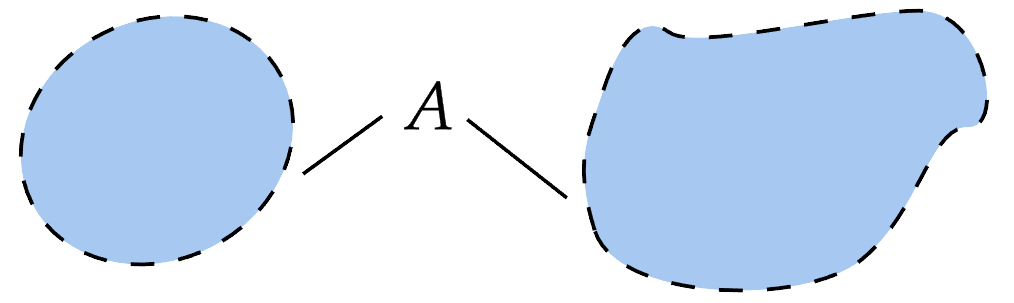
\includegraphics[width=0.5\textwidth]{fig/7.9.png}
        \captionof{figure}{$\mb{E}^n$的开子集不是道路连通的}
    \end{center}
\end{instance}

\begin{instance}
    令 $X=\{(x,y)\in\mathbb{E}^2\mid x\in\mathbb{Q}\text{ 或 }y=0\}$.
    \begin{center}
        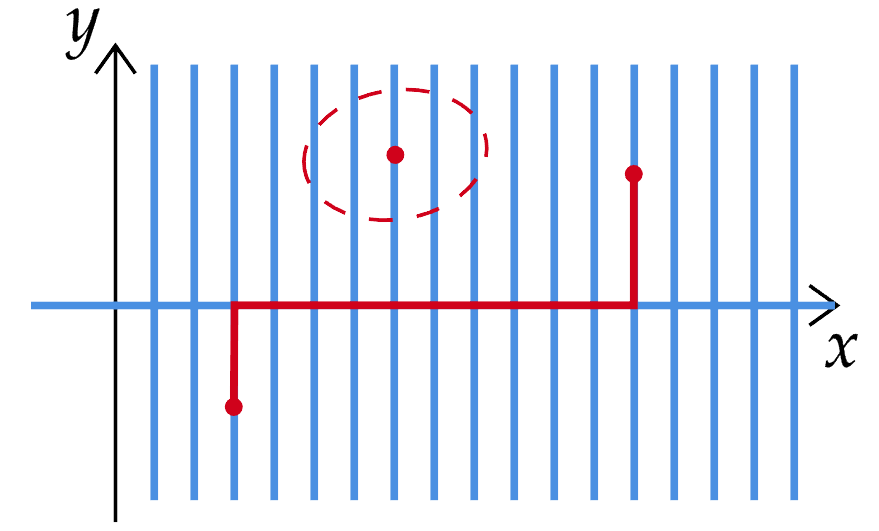
\includegraphics[width=0.4\textwidth]{fig/7.10.png}
        \captionof{figure}{}
    \end{center}\par
    直接由图像可以看出它是道路连通的，但并非局部道路连通的.
\end{instance}

上述例子告诉我们局部道路连通空间可能并非道路连通.同样地，道路连通空间可能并非局部道路连通的情况，因此道路连通和局部道路连通是既不充分也不必要的两个条件.此外，还有既不是道路连通也不是局部道路连通的例子.\par

\begin{instance}
    拓扑学家正弦曲线 $X$ 不是局部道路连通的.\par
    在$\left(0,\frac{1}{2}\right)$ 附近的任何小邻域都包含 $A$ 与 $B$ 的“振荡”部分，因此均为不相交的斜线，因此无法找到包含$\left(0,\frac{1}{2}\right)$的道路连通开邻域.
\end{instance}

下面这个命题告诉我们连通集补充上局部道路连通的性质后就是一个道路连通集.
\begin{proposition}[连通且局部道路连通蕴含道路连通]
    若 $X$ 连通且局部道路连通，则 $X$ 道路连通.
\end{proposition}
\begin{proof}
    反证法，假设$X$是连通的，局部道路连通的但不是道路连通的.\par
    则$X$可分解为互不相交的道路连通开集族 $X=\bigcup_{\lambda\in\Lambda}\{P_\lambda\},|\Lambda|\geq 2$.\par
    任取$P_{\lambda_0}$，$\forall\, x\in P_{\lambda_0}$，由于$X$局部道路连通，故$x$存在一个道路连通邻域$V$，就有$V\subset P_{\lambda_0}$.因此$P_{\lambda_0}$是开集.\par
    类似地，$\forall\,\lambda\in\Lambda$，$P_\lambda$是开集，因此$\bigcup_{\lambda\neq\lambda_0}{P_\lambda}$是开集.\par
    因此，$\bigcup_{\lambda\neq\lambda_0}{P_\lambda}$的补集$P_{\lambda_0}$是开集，故 $P_{\lambda_0}$为既开又闭的非空真子集，与$X$连通矛盾.
\end{proof}

\begin{corollary}
    若 $A\subset \mathbb{E}^n$ 是开集且连通，则$A$道路连通.
\end{corollary}

\section{区分拓扑空间}

\begin{lemma}[限制仍为同胚]
    若 $f:X\to Y$ 是同胚，$A\subset X$，则限制 $f|_A:A\to f(A)$ 也是同胚.
\end{lemma}
\begin{proof}
    只需证明$f|_A$是连续的，开的双射.其中连续双射由$f$的性质直接可得，因此只需证明$f|_A$是开映射.\par
    设$U\subset A$是$X$中的开集，则$U\cap A$是$A$中开集.\par
    由于$f$是双射，$f(U\cap A)=f(U)\cap f(A)$，且$f(U)$是$Y$中的开集，因此$f(U\cap A)=f(U)\cap f(A)$在$f(A)$中开.\par
    故$f$为开映射.
\end{proof}

\begin{instance}
    $\mathbb{E}^1\not\cong \mathbb{E}^n$$(n\geq 2)$.\par
    若存在同胚 $f: \mathbb{E}^1\to\mathbb{E}^n$，取一点 $p\in \mathbb{E}^1$.则 $\mathbb{E}^1\setminus\{p\}$ 不连通，而 $\mathbb{E}^n\setminus\{f(p)\}$ 连通(对 $n\geq 2$).\par
    由限制同胚引理得到 $f|_{\mathbb{E}^1\setminus\{p\}}:\mathbb{E}^1\setminus\{p\}\to \mathbb{E}^n\setminus\{f(p)\}$ 同胚.由于连通性为拓扑不变量.矛盾.
\end{instance}

\begin{instance}
    $S^1\not\cong S^n(n\ge 2)$.\par
    若 $f:S^1\to S^n$ 为同胚，取点 $p\in S^1$.则 $S^1\setminus\{p\}$ 同胚于 $\mathbb{E}^1$，而 $S^n\setminus\{f(p)\}$ 同胚于 $\mathbb{E}^n$.同样由限制同胚引理导出矛盾.
\end{instance}































